\documentclass[aspectratio=169]{beamer}
%[handout]

\usetheme[progressbar=frametitle]{metropolis}
\usepackage{appendixnumberbeamer}

\usepackage[utf8]{inputenc}
\usepackage[T1]{fontenc}

\usepackage[brazil]{babel}
\usepackage[outputdir=..]{minted}
\usepackage{xcolor}
\usepackage{soul} % strikethrough
\usepackage{advdate}
\usepackage{graphicx}
\graphicspath{{figs/}}
\usepackage{graphbox}

\usepackage[ampersand]{easylist}

\usepackage{multirow}
\usepackage{multicol}
\usepackage{subcaption}

\usepackage{pgf,tikz}
\usetikzlibrary{shapes,arrows,positioning}
\usetikzlibrary{circuits.logic.US}
\usetikzlibrary{matrix,calc}

\usepackage{karnaugh-map}

\usepackage{pgfpages}
\setbeameroption{hide notes} % Only slides
% \setbeameroption{show only notes} % Only notes
% \setbeameroption{show notes on second screen=right} % Both

% \graphicspath{{../figs/}}

\definecolor{bgc}{rgb}{0.95,0.9,0.95}
\definecolor{links}{HTML}{2A7F7F}
\hypersetup{colorlinks,linkcolor=,urlcolor=links}

\newminted{verilog}{fontsize=\scriptsize, 
    linenos,
    numbersep=8pt,
    bgcolor=bgc,
    tabsize=4,
    framesep=3mm} 
    %frame=lines,

\newcommand{\verilog}[1]{\verilogf{#1}{\footnotesize}}

\newcommand{\verilogf}[2]{\inputminted[fontsize=#2, 
    linenos,
    tabsize=2,
    numbersep=4pt,
    bgcolor=bgc,
    framesep=3mm]{verilog}{../codes/#1.v}
}

\newminted{nasm}{fontsize=\scriptsize, 
		   linenos,
		   numbersep=8pt,
           bgcolor=bgc,
		   framesep=3mm} 

\usepackage{booktabs}
\usepackage[scale=2]{ccicons}

\usepackage{pgfplots}
\usepgfplotslibrary{dateplot}

\usepackage{hyperref}


\usepackage{xspace}
\newcommand{\themename}{\textbf{\textsc{metropolis}}\xspace}



\usepackage{pifont}% http://ctan.org/pkg/pifont
\newcommand{\cmark}{\ding{51}}%
\newcommand{\xmark}{\ding{55}}%

% \tiny	
% \scriptsize
% \footnotesize
% \small	
% \normalsize	
% \large	
% \Large	
% \LARGE	
% \huge	
% \Huge	



\newminted{python}{fontsize=\scriptsize, 
		   linenos,
		   breaklines,
		   numbersep=8pt,
           tabsize=2,
		   framesep=3mm} 
		   
\newminted{verilog}{fontsize=\scriptsize, 
		   linenos,
		   breaklines,
		   numbersep=8pt,
           tabsize=2,
		   framesep=3mm} 
		   




\definecolor{bgc}{rgb}{0.95,0.9,0.95}
\definecolor{links}{HTML}{2A7F7F}
\hypersetup{colorlinks,linkcolor=,urlcolor=links}


% \usepackage[style=apa]{biblatex}
% \addbibresource{mm.bib}


% \author{\large Prof. Ricardo Menotti (\href{mailto:menotti@ufscar.br}{menotti@ufscar.br})}

\newcommand{\newauthor}[2]{
  \parbox{0.50\textwidth}{
    \texorpdfstring
      {
        \centering
        \small #1 \newline
        {\scriptsize{\urlstyle{same}\href{mailto:#2}{#2}\urlstyle{tt}}}
      }
      {#1} \newline
  }
}

\author{
  \newauthor{Prof. Ricardo Menotti}{menotti@ufscar.br}
\and \newauthor{Prof. Luciano de Oliveira Neris}{lneris@ufscar.br}  
%\and \newauthor{Prof. Artino Quintino da Silva Filho}{artino@ufscar.br}
% \and \newauthor{Prof. Maurício Figueiredo}{mauricio@ufscar.br}
% \and \newauthor{Prof. Edilson Kato}{kato@ufscar.br}
% \and \newauthor{Prof. Roberto Inoue}{rsinoue@ufscar.br}
}

\date{Atualizado em: \today}

\institute{\large \textbf{Departamento de Computação} \\
Centro de Ciências Exatas e de Tecnologia \\
Universidade Federal de São Carlos}

\title{Lógica Digital (1001351)}

\titlegraphic{\hfill
\includegraphics[height=1.5cm]{LogoUfscar}}



\subtitle{Mapas de Karnaugh} % 

% https://tex.stackexchange.com/questions/140567/drawing-karnaughs-maps-in-latex
% http://www.texample.net/tikz/examples/karnaugh-diagram/

\begin{document}

\begin{frame}
	\titlepage
\end{frame} 

%%%%%%%%%%%%%%%%%%%%%%%%%%%%%%%%%%%%%%%%%%%%%%%%%%%%%%%%%%%%%%%%%%%%%%%%%%%%%%%%

\section{Mapas de Karnaugh}

\frame{     \centering
    \frametitle{\insertsection}
\begin{tikzpicture}
\tikzstyle{foo} = [-latex, cyan, ultra thick, rounded corners]
\tikzstyle{bar} = [-latex, magenta, ultra thick, rounded corners]
\node[anchor=south west,inner sep=0](image) at (0,0){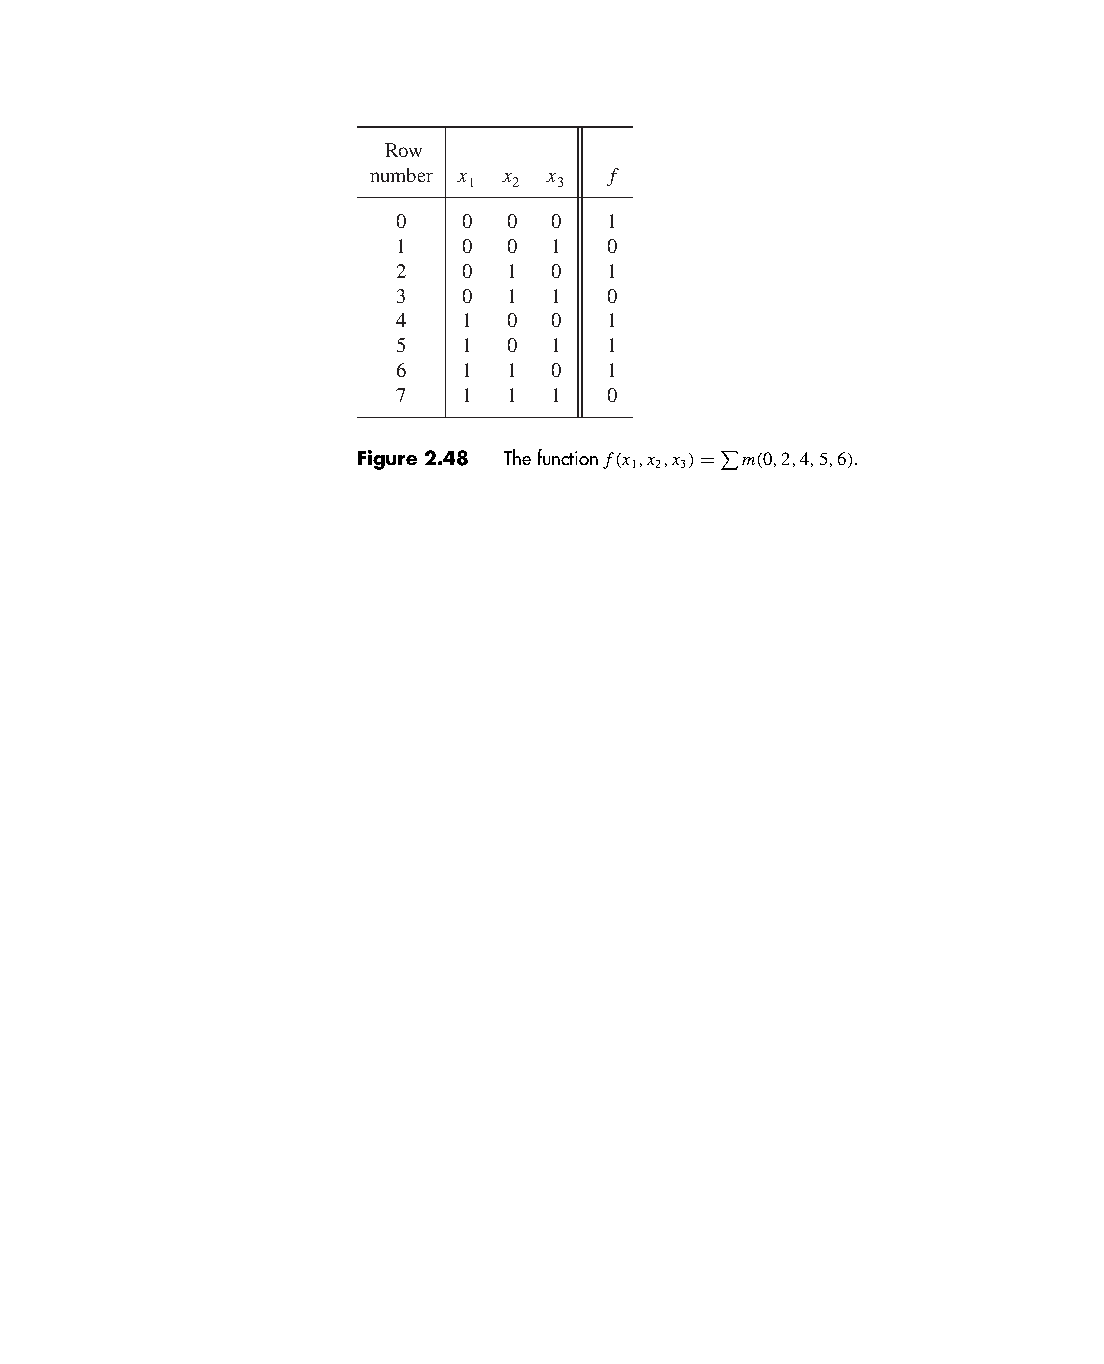
\includegraphics{VerilogFig2_48}};
% \draw[step=0.25cm,gray,very thin] (0,0) grid (9,6);
% \draw[step=1cm,black,very thin] (0,0) grid (9,6);
\onslide<2,4->{
\draw[bar] (3.7, 4.5)   to (4.3, 4.5); 
\draw[bar] (3.7, 3.6)   to (4.3, 3.6); 
\draw[bar] (3.7, 2.75)  to (4.3, 2.75); 
\draw[bar] (3.7, 1.875) to (4.3, 1.875); 
\node[bar](x3) at (5,5.125) {$=\overline{x}_3$};
}
\onslide<3,4->{
\draw[foo] (3, 2.75)  to (4.3, 2.75); 
\draw[foo] (3, 2.3)  to (4.3, 2.3); 
\node[foo](x1x2) at (6,5.125) {$+x_1\overline{x}_2$};
}
\onslide<4->{
\draw[bar, blue] (3.7, 2.75)  to (4.3, 2.75); 
}
\onslide<5-> {
    \node[anchor=south west,inner sep=0](a) at (7,4){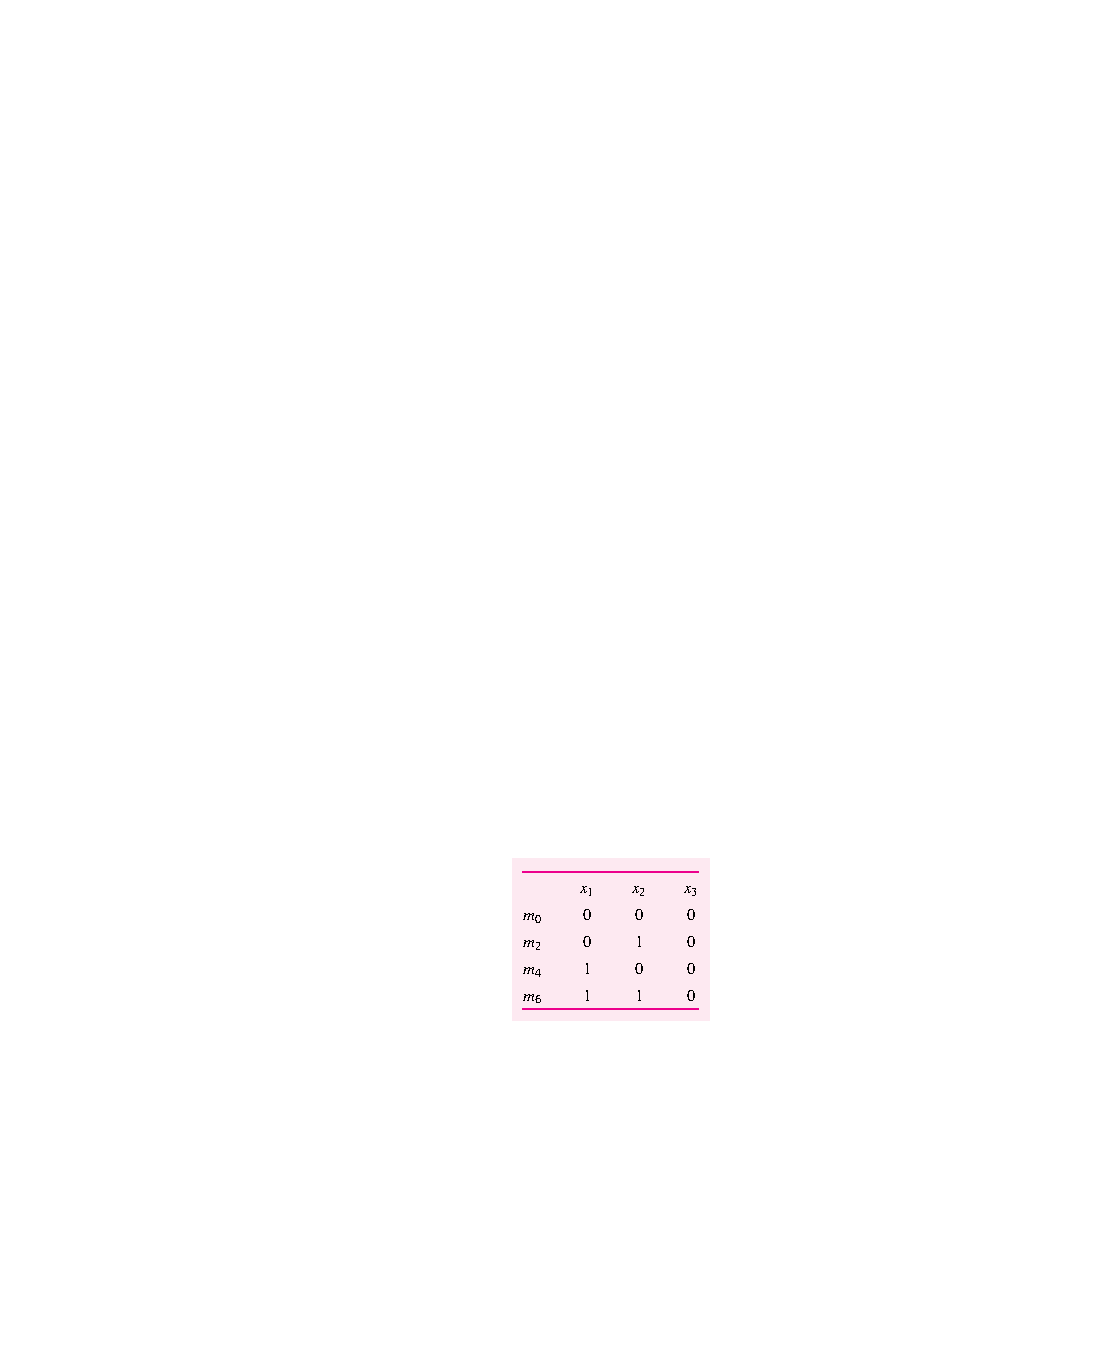
\includegraphics{VerilogFig2_48a}};
    \node[anchor=south west,inner sep=0](b) at (7,2){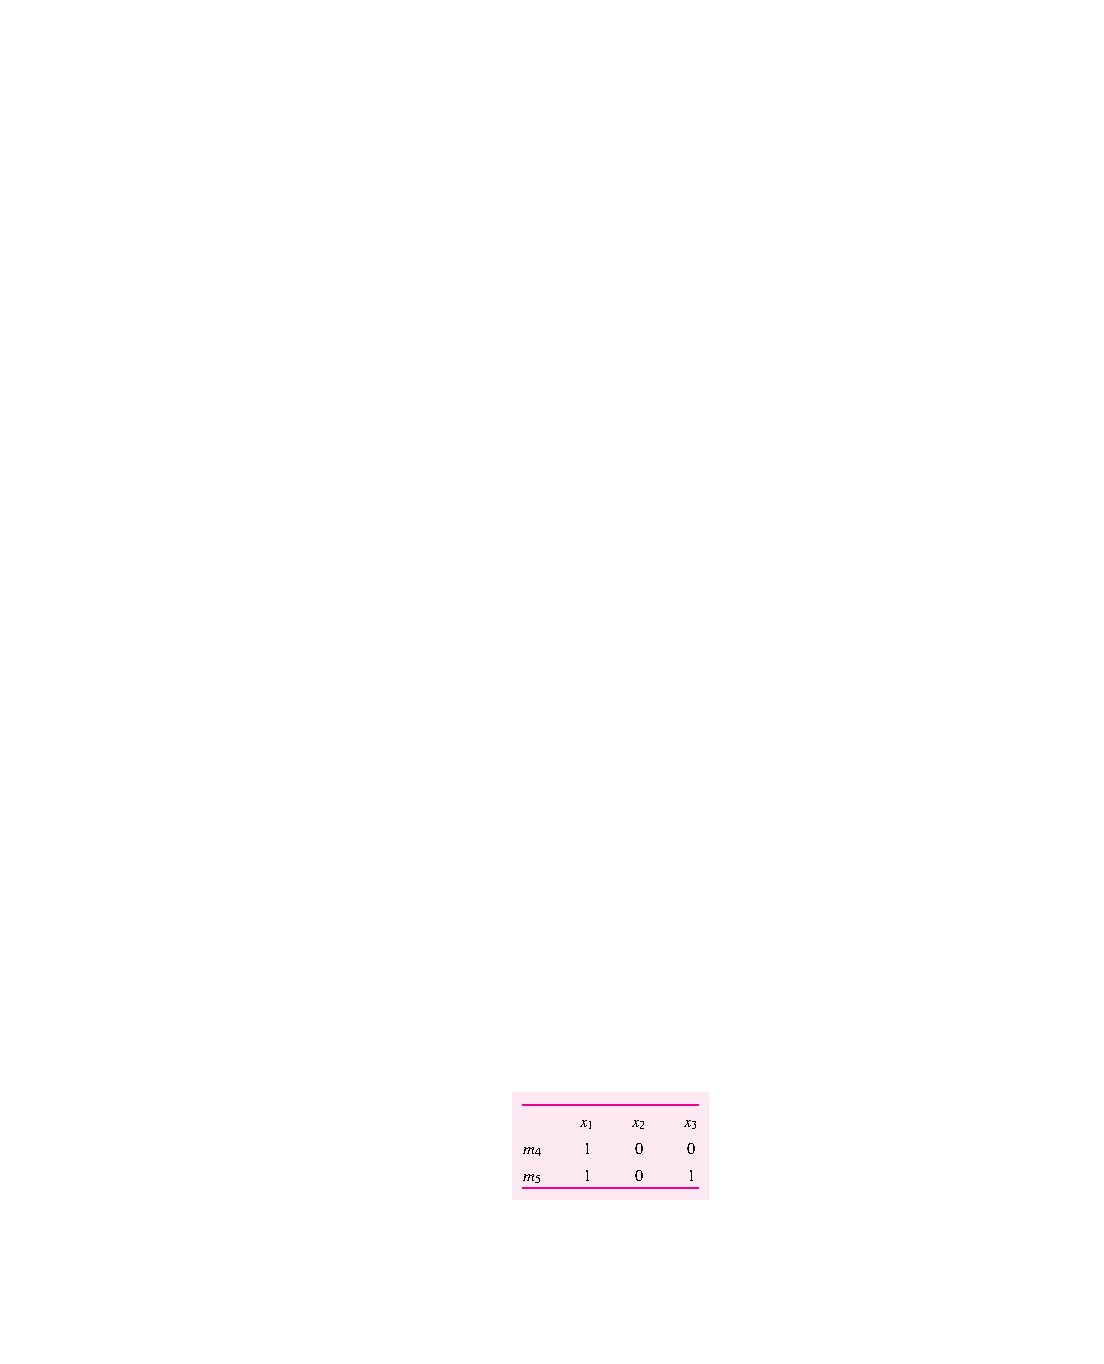
\includegraphics{VerilogFig2_48b}};
    \draw[bar] (x3) to[bend left] (a);
    \draw[foo] (x1x2) to[bend right] (b);
}
\end{tikzpicture}%
}

\begin{frame}{\insertsection: duas variáveis} \centering
    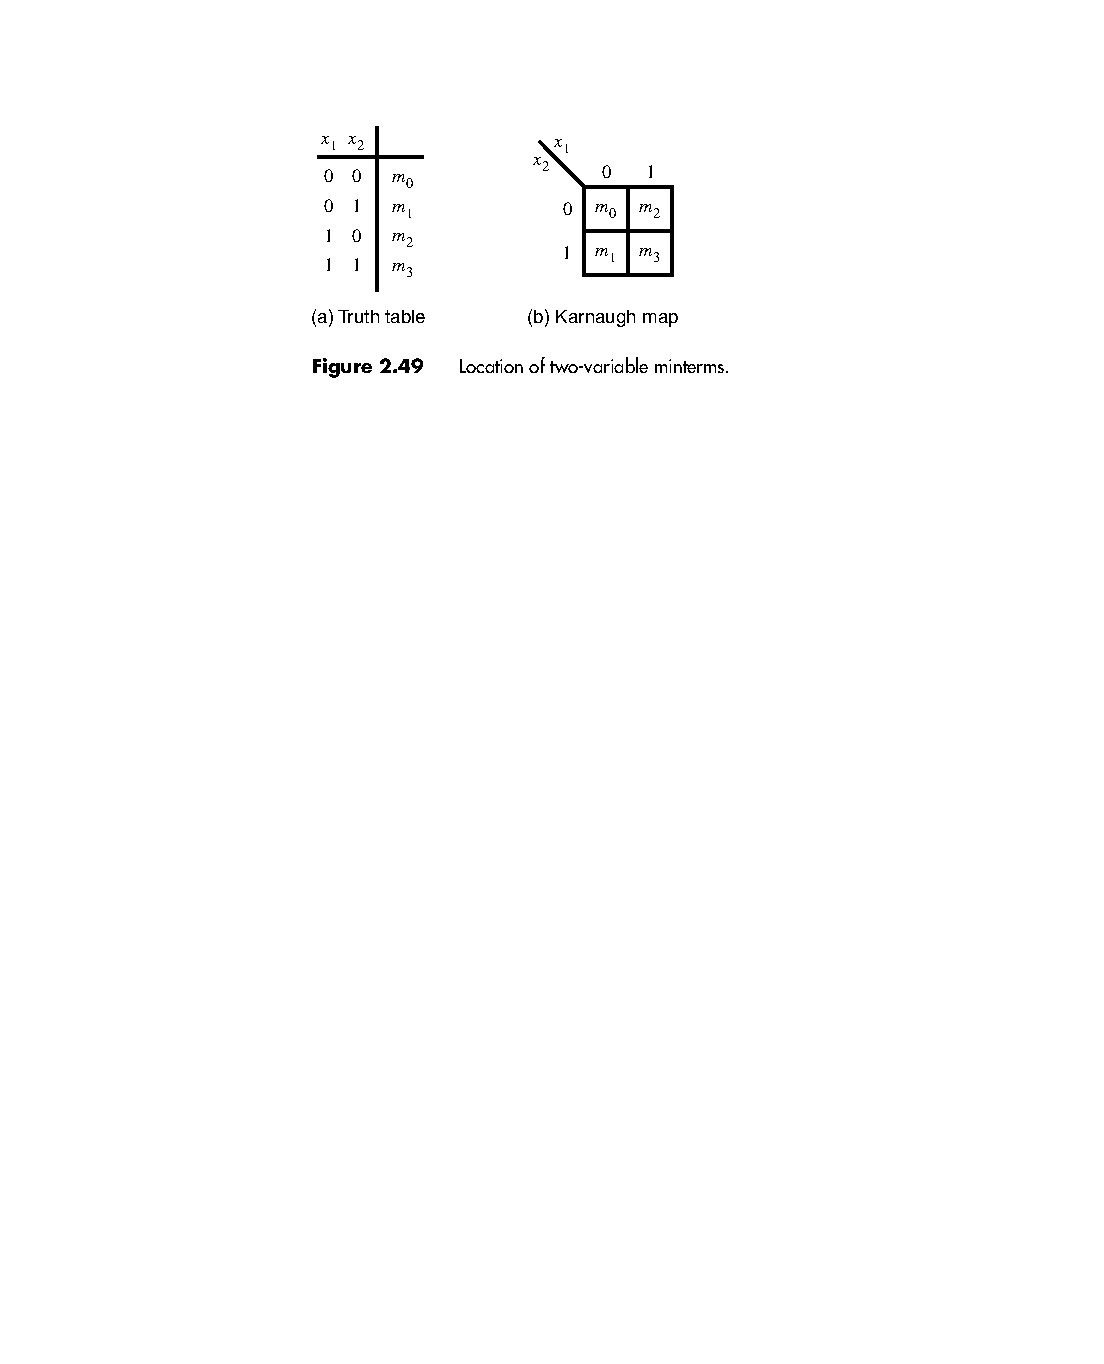
\includegraphics[width=.6\textwidth]{VerilogFig2_49}
    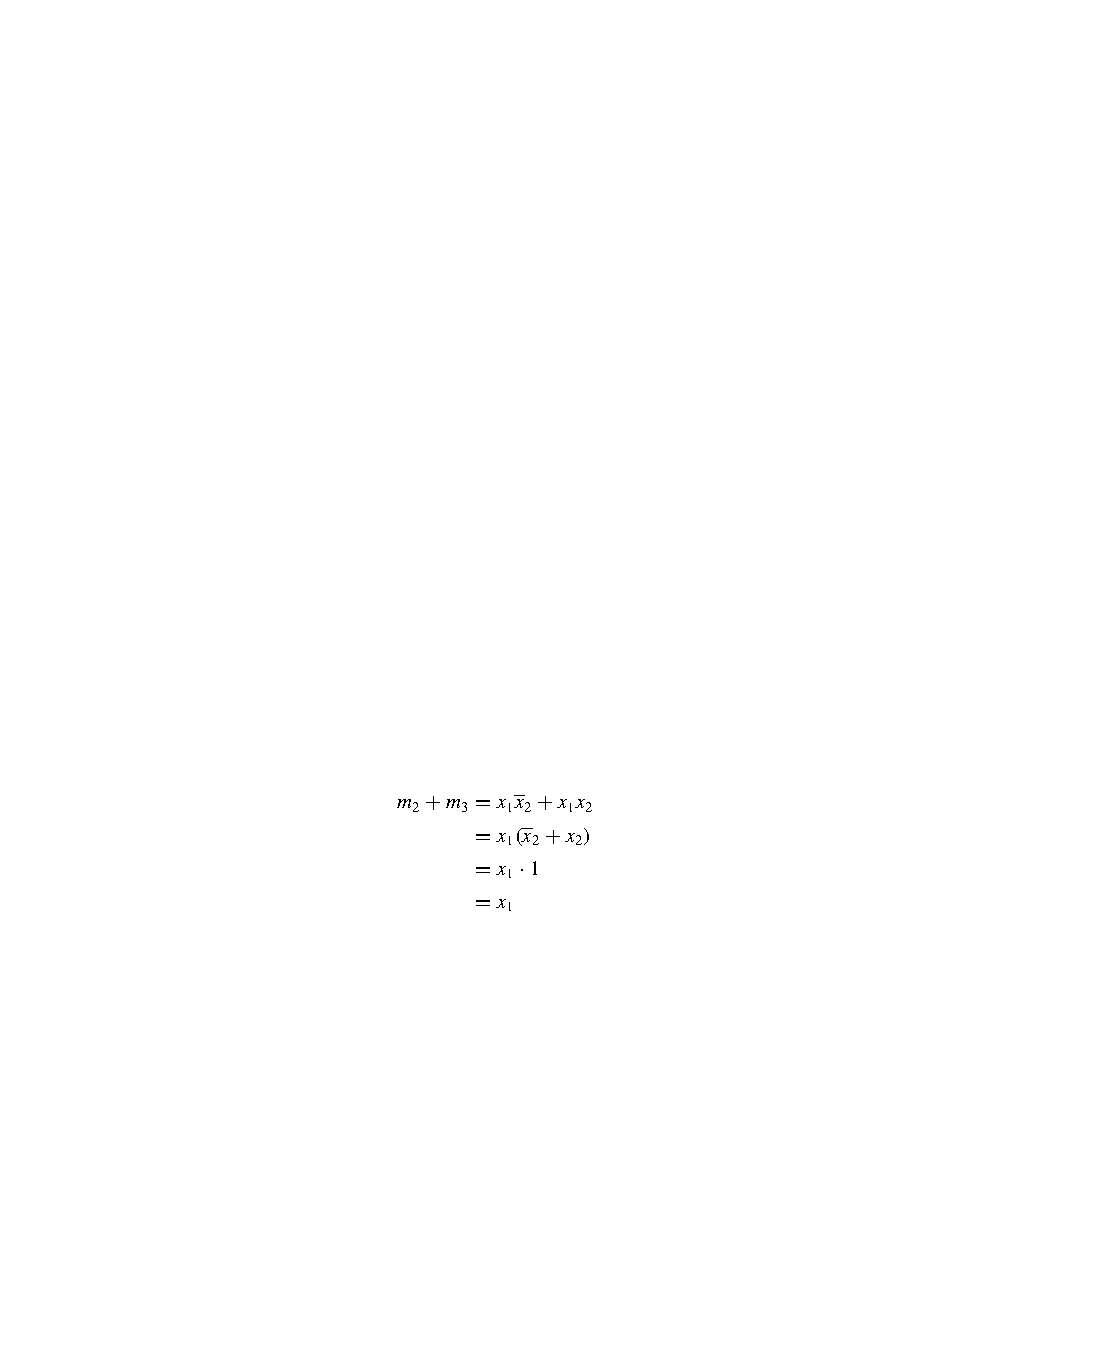
\includegraphics[width=.3\textwidth]{VerilogFig2_49a}
\end{frame}

\begin{frame}{\insertsection: duas variáveis} \centering
    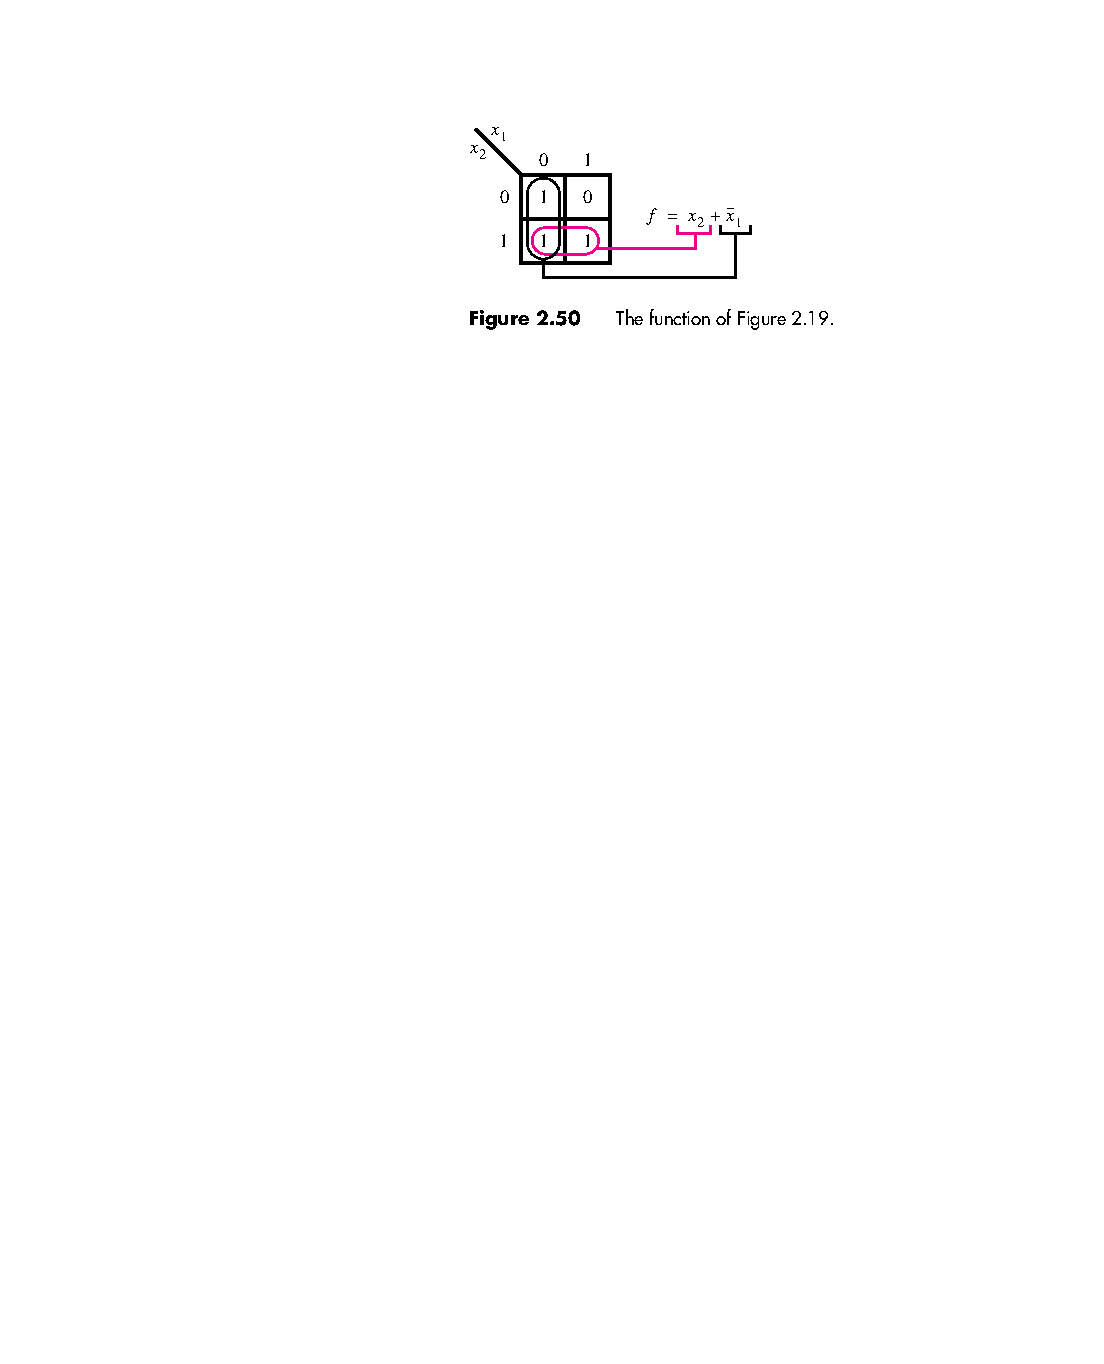
\includegraphics[width=.6\textwidth]{VerilogFig2_50}
\end{frame}

\begin{frame}{\insertsection: três variáveis} \centering
    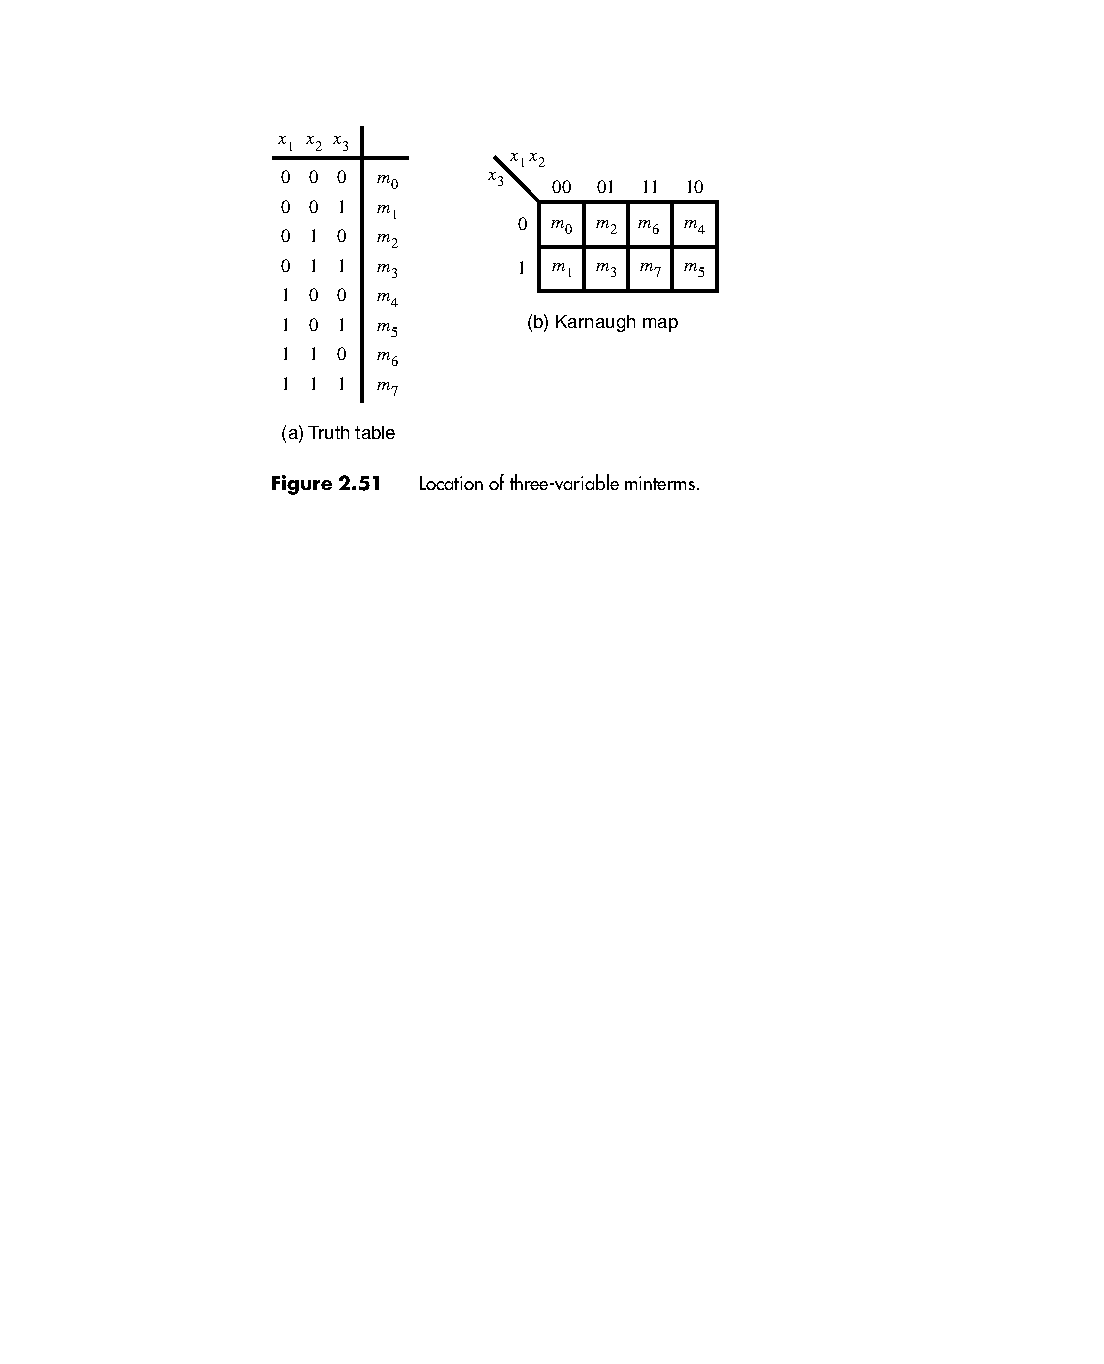
\includegraphics[width=.8\textwidth]{VerilogFig2_51}
\end{frame}

\begin{frame}{\insertsection: três variáveis} \centering
    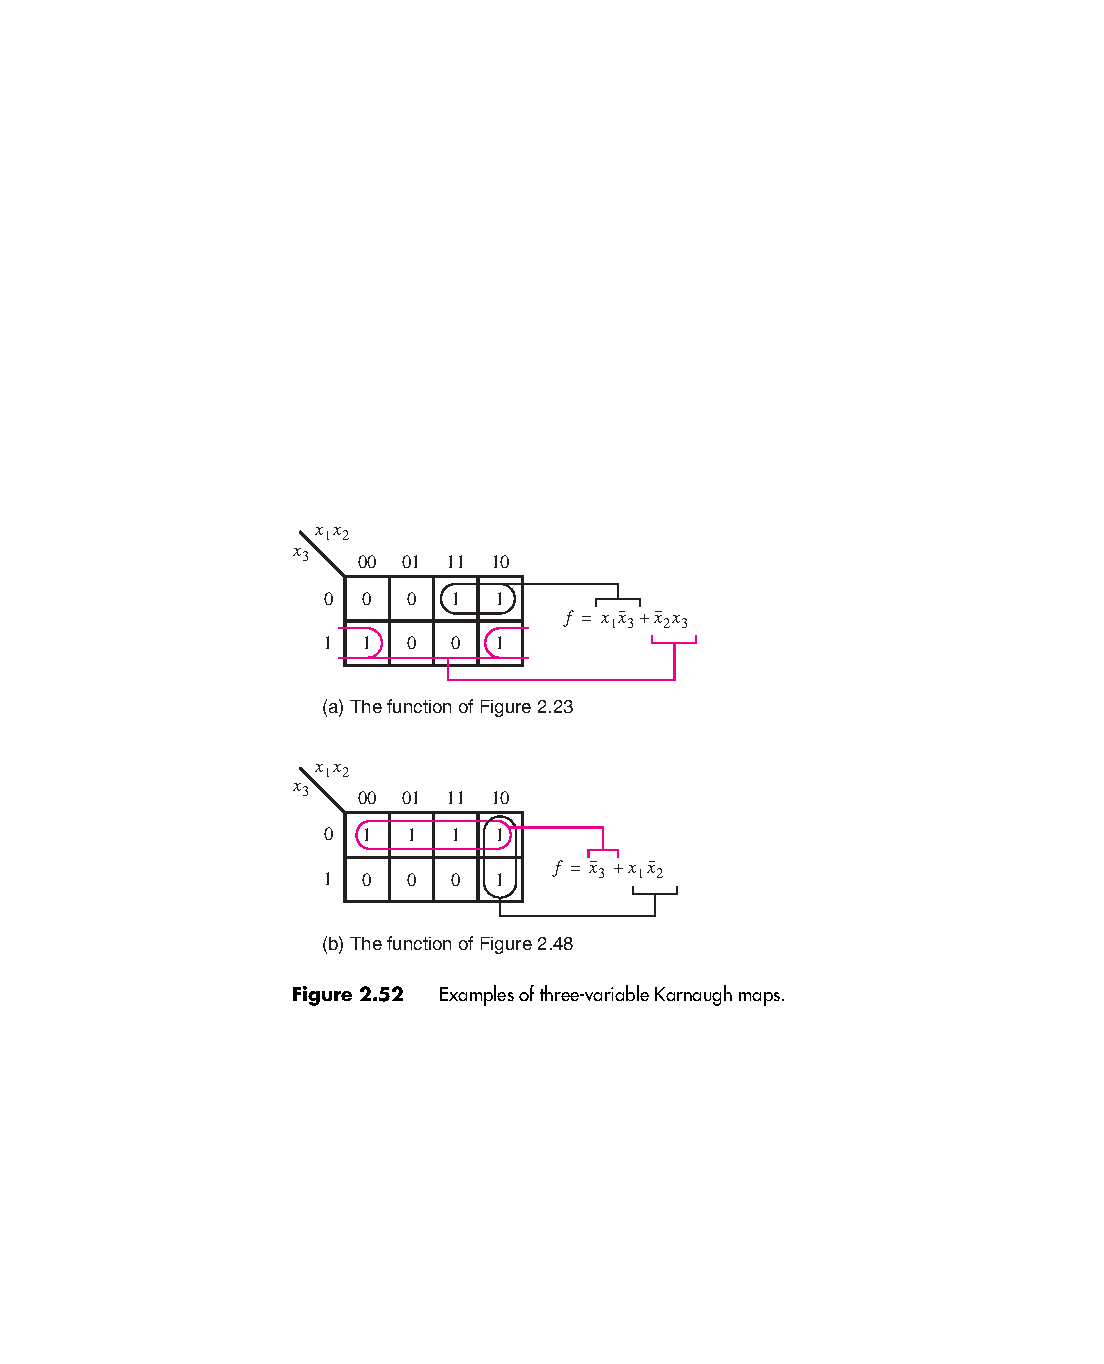
\includegraphics[width=.65\textwidth]{VerilogFig2_52}
\end{frame}

\begin{frame}{\insertsection: quatro variáveis} \centering
    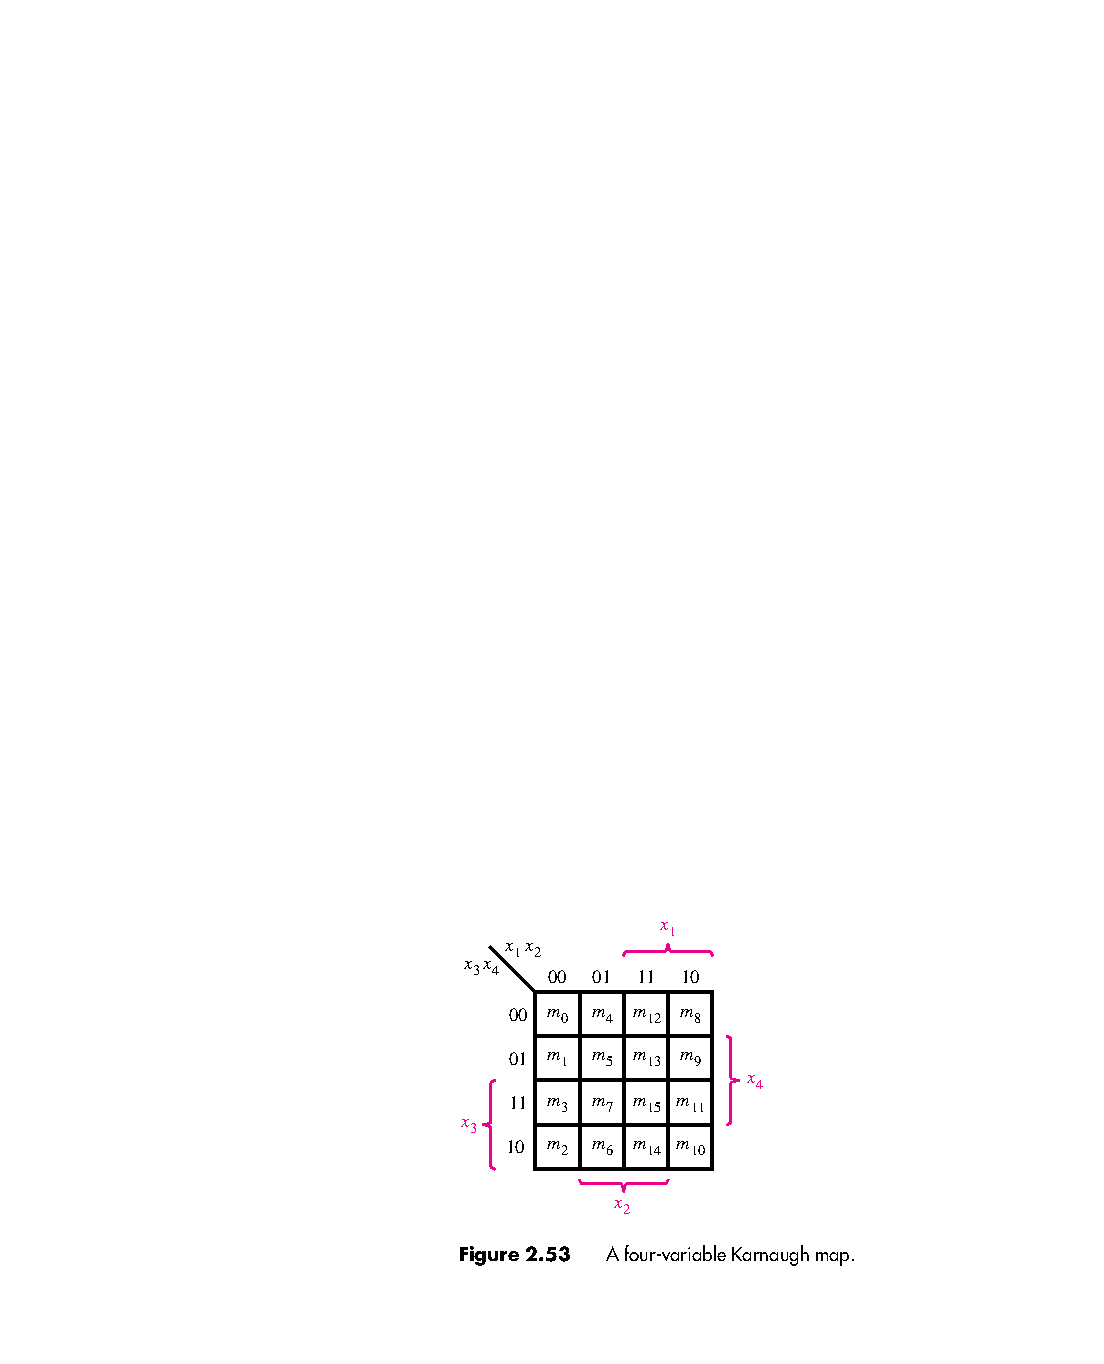
\includegraphics[width=.7\textwidth]{VerilogFig2_53}
\end{frame}

\begin{frame}{\insertsection: quatro variáveis} \centering
    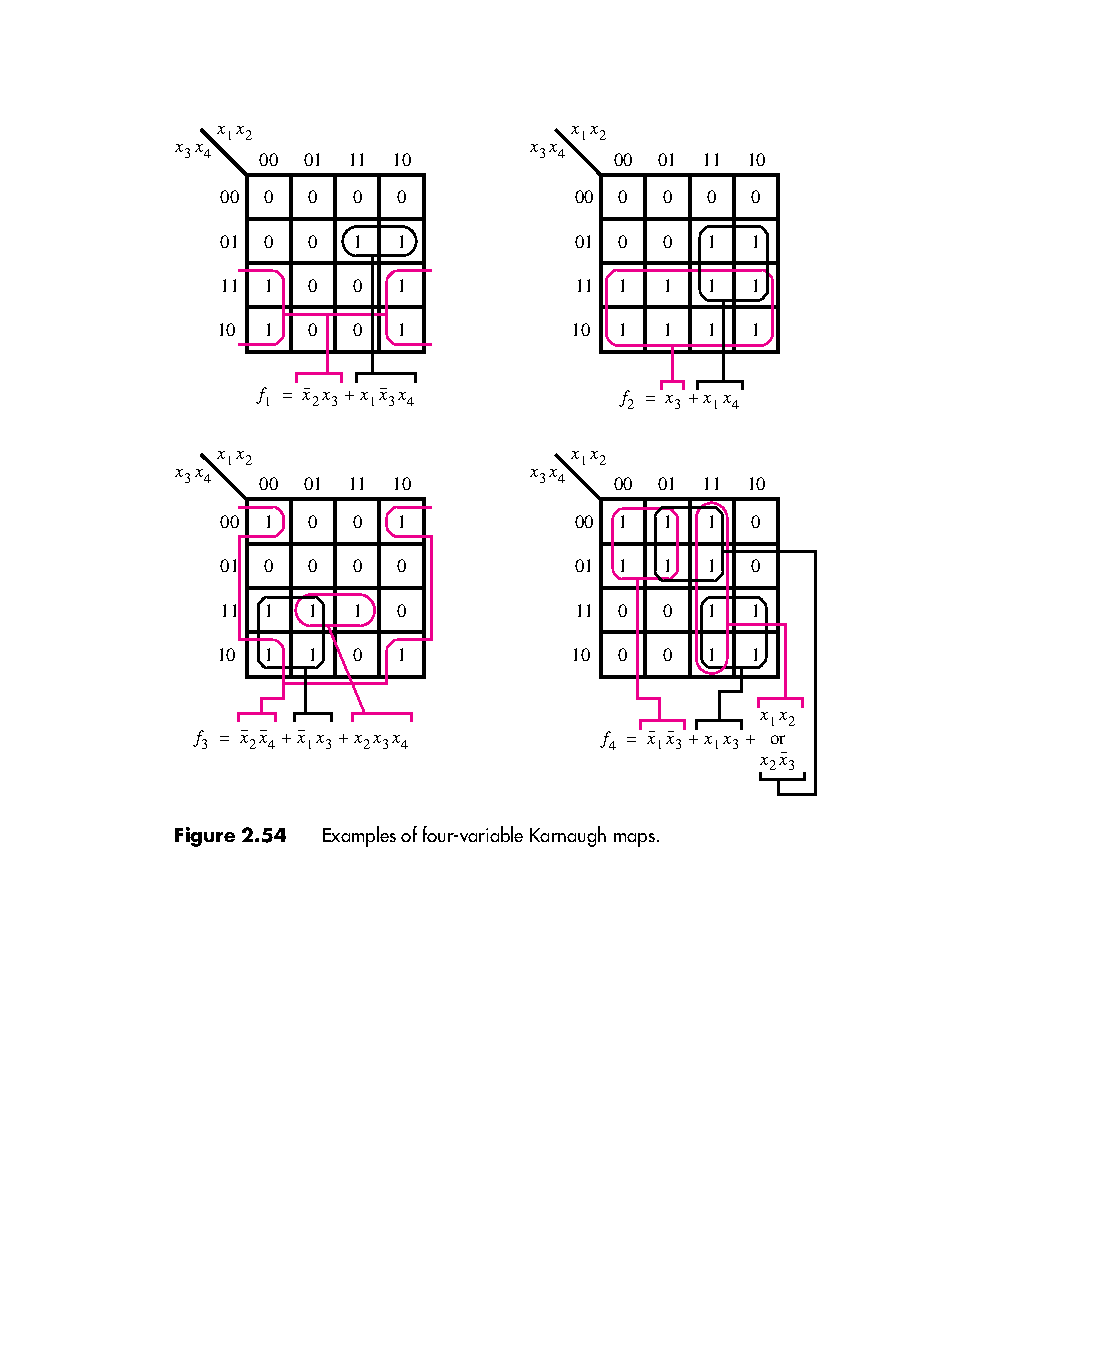
\includegraphics[width=.55\textwidth]{VerilogFig2_54}
\end{frame}

\begin{frame}{\insertsection: cinco variáveis} \centering
    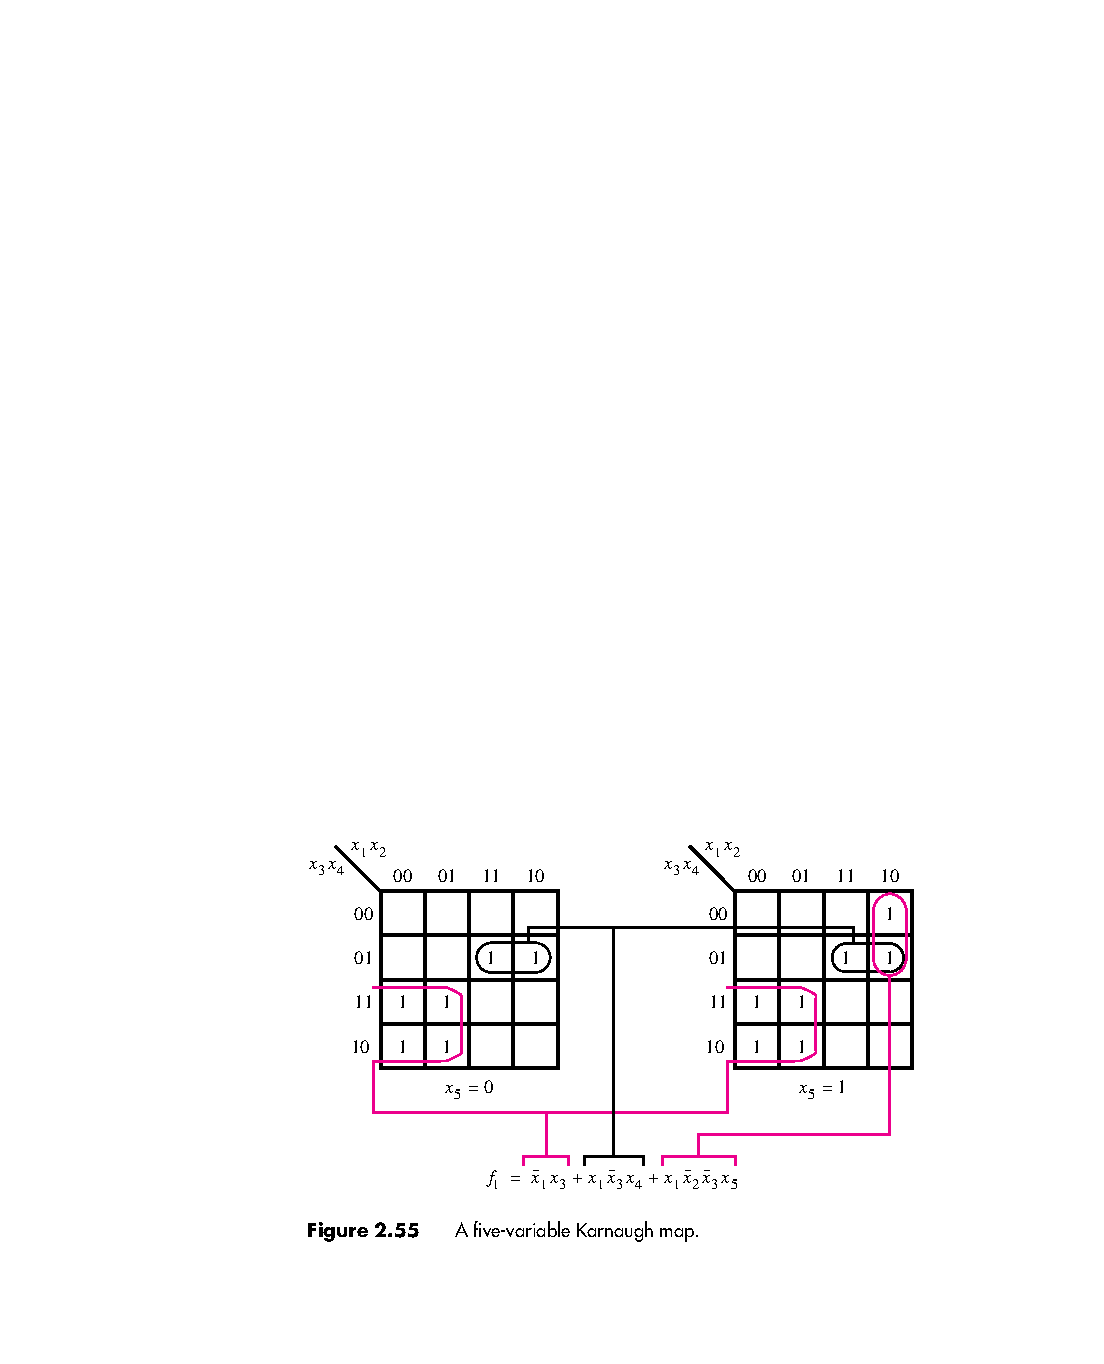
\includegraphics[width=.8\textwidth]{VerilogFig2_55}
\end{frame}

\section{Bibliografia} %%%%%%%

\begin{frame}{\insertsection} 
	\begin{itemize}
		\item \href{https://www.google.com.br/search?q=filetype\%3Apdf+Fundamentals+of+Digital+Logic+with+Verilog+Design+&oq=filetype\%3Apdf}{Brown, S. \& Vranesic, Z. - Fundamentals of Digital Logic with Verilog Design, 3rd Ed., Mc Graw Hill, 2009}
	\end{itemize}
\end{frame}

\begin{frame}
	\titlepage
\end{frame} 

\end{document}